\documentclass{SBCbookchapter}
\usepackage[utf8x]{inputenc}
\usepackage[T1]{fontenc}
\usepackage[brazilian]{babel}
\usepackage{graphicx}
\usepackage{hyperref}

\hyphenpenalty=5000
\tolerance=1000


\title{Tolerância a Falhas na Computação Ubíqua}
\author{Cícero Camargo}

\begin{document}
\maketitle

% \begin{abstract}
% The book is on the table
% \end{abstract}

\begin{resumo}

O conceito de computação ubíqua abre um leque de possíveis aplicações, nas quais diversos recursos computacionais estarão distribuídos e integrados no ambiente físico. Aplicações diretas da computação ubíqua têm surgido em ambientes inteligentes e de monitoramento médico, por exemplo. No entanto, para que soluções com esse perfil surjam, de fato, na indústria, estas devem ser não intrusivas e altamente confiáveis, ou, do contrário, seu uso pode gerar desde simples incômodos aos usuários até riscos de morte. Tolerância a falhas é uma peça-chave na construção de um sistema ubíquo, porém as características da ubiquidade complicam ainda mais os possíveis cenários de falhas. Contudo, embora este seja um assunto recente na computação ubíqua, diversas discussões e soluções tem sido propostas na academia. Este busca revisar trabalhos já consolidadas, bem como revisar o estado da arte das técnicas de tolerância a falhas na computação ubíqua.

\end{resumo}

%\tableofcontents

\section{Introdução} % (fold)

A computação ubíqua anuncia uma nova era, a qual já começamos a vivenciar, onde diversos dispositivos computacionais estão completamente integrados com o ambiente e interconectados de forma que os usuários podem acessar seus dados e aplicações com diversos níveis de transparência. A sustentabilidade da computação pervasiva depende que a complexidade da infraestrutura de software e hardware esteja escondida do usuário final. Em um ambiente onde dispositivos de rede, computadores pessoais, sensores, entre outros dispositivos, devem ser integrados de forma transparente ao usuário, as diversas falhas que podem ocorrer são exemplos destas complexidades que devem ser abstraídas ou contornadas sempre que possível.

Tolerância a falhas é um tema ainda pouco abordado no âmbito dos sistemas ubíquos, porém é um conceito primordial para que acomputação ubíqua ganhe espaço, pois uma vez que tais sistemas devem residir no mesmo meio físico (e virtual) dos usuários, falhas podem ser irritantes e, até mesmo, uma ameaça a vidas humanas. Diversos pesquisadores da área argumentam que as técnicas atuais de tolerância a falhas devem ser repensadas para o contexto ubíquo. Em~\cite{Banavar2000} o autor reafirma a necessidade de proteger um sistema contra falhas para ser aplicado em casas inteligentes. Discussão semelhante é apresentada em~\cite{Bohn02} onde o autor expressa os requisitos de tolerância a falhas específicos de ambientes de monitoramento na área médica.

A computação ubíqua tem encontrado sua aplicação direta na área médica\linebreak\cite{Bang03} e em espaços inteligentes (\emph{smart spaces})~\cite{Kidd99} onde sensores são usados para monitorar pacientes em um hospital, identificar distúrbios da idade em idosos ou capturar o estado de instalações elétricas em cômodos inteligentes. Neste cenário de aplicação, a ocorrência de falhas pode accaretar em sérias consequências, incluindo o risco de morte de usuários. Logo, tolerância a falhas é uma questão vital.

As falhas também abrem novas situações com diferentes implicações no contexto de sistemas ubíquos. Por exemplo, falhas podem resultar em inferências incorretas de informação, levando a falhas de segurança, privacidade e acesso indevido de recursos. Logo, a contenção de falhas é um aspecto de grande importância em um sistema ubíquo para uso comercial.

O objetivo deste capítulo é apresentar os principais desafios relacionados a tolerância a falhas dentro da computação ubíqua, bem como apresentar diversas estratégias já propostas e implementadas em ambientes e ferramentas de computação ubíqua desenvolvidas por grupos de pesquisa.

Em ~\emph{``\nameref{sec:falhas_comp}''} serão introduzidos diversos conceitos consolidados sobre tolerância a falhas na computação como uma grande área. \emph{``\nameref{sec:falhas_ubicomp}''} apresenta os principais desafios de tolerância a falhas encontrados pelos pesquisadores da computação ubíqua em específico. Em \emph{``\nameref{sec:tolerancia}''} são apresentados alguns avanços de pesquisa em direção a uma computação ubíqua tolerante a falhas. A Seção~\emph{``\nameref{sec:estudos}''} mostra o que tem sido aplicado de soluções práticas de tolerância a falhas em ferramentas e ambientes de computação ubíqua. Em \emph{``\nameref{sec:conclusoes}''} é discutido o estado atual desta sub-área e os avanços críticos em tolerância a falhas que, acredita-se, devam surgir para que a computação ubíqua avance como um todo e mais soluções apareçam no mercado, para o usuário final.

% section introducao (end)

\section{Tolerância a falhas na computação}
\label{sec:falhas_comp}
Confiabilidade e disponibilidade são características altamente desejadas em sistemas de computação, pois a humanidade depende cada vez mais de sistemas automatizados e informatizados para a realização de suas tarefas diárias. Dentre estes estão sistemas críticos, como um sistema que envolva transações financeiras ou software controlador de um avião, por exemplo, onde falhas podem causar prejuízo financeiro e/ou perda de vidas.

Os computadores (hardware + software) são, provavelmente, os sistemas mais complexos já inventados pelo homem. A complexidade das peças de hardware segue em constante crescimento, o que gera a possibilidade de inserção de defeitos em várias etapas do desenvolvimento, desde o nível elétrico até, por exemplo, algoritmos de predição implementados diretamente em hardware nos processadores. A área de software é ainda mais complexa e, por isso, ainda mais propensa a falhas. Até mesmo o ônibus espacial (\emph{Space Shuttle}) da NASA~\cite{BonacheaOnline}, desenvolvido com as mais cuidadosas tecnologias apresentou \emph{bugs} no código de seu sistema sistema, podendo resultar em uma catástrofe. Podemos extrapolar um pouco e afirmar que falhas são inevitáveis em computadores. Contudo, as consequências dessas falhas pode ser contornadas ou, ao menos minimizadas, se o design do software se prevenir das falhas que possam vir a ocorrer no sistema.

É notável o crescimento em confiabilidade na área de hardware~\cite{Weber} onde vimos uma grande cultura de tolerância a falhas se formar dos inseguros \emph{mainframes} a vávula, cujos proprietários sofriam, rotineiramente, com falhas de diversas origens, até os robustos \emph{laptops} (e \emph{smartphones}) que temos hoje para computação pessoal. Na área de software, por outro lado, os processos de desenvolvimento e os produtos estão cada vez mais complexos e apresentando cada vez mais \emph{bugs}. Uma vez que esses \emph{bugs} são quase inevitáveis, mecanismos de tolerância a falhas se tornam obrigatórios em sistemas onde a confiabilidade e disponibilidade é imprescindível.

\subsection{Falhas, erros e defeitos} % (fold)
\label{sub:falhas_erros_e_defeitos}

Com frequência usamos as palavras ``falha'', ``erro'' e ``defeito'' para designar problemas que fazem um módulo de software ou hardware funcionar de forma indevida. Contudo, na área de tolerância a falhas faz-se uma distinção destes três termos. Diversos autores da área possuem definições sutilmente diferentes para esses termos, e as definições que usaremos aqui são as mesmas econtradas em~\cite{koren2007fault}.

Uma \textbf{falha}, do inglês \emph{fault} (também traduzido como \textbf{falta}), ou \textbf{defeito} (\emph{failure}) pode ser algum problema diretamente no hardware ou algum \emph{bug} na programação do software. Já o \textbf{erro} é uma manifestação de uma falha.

Por exemplo, considere um circuito que faz a soma de dois números binários, porém com um dos bits de saída preso em $0$ (zero), independente da soma dos operandos. Este defeito ou falha no hardware só gerará um erro quando a soma dos operandos resultar em um valor em que aquele bit específico da saída não seria igual a zero. Outro exemplo, na área de software, é uma linha de código mal programada, a qual pode eventualmente acessar uma área de memória inválida. Esta falha de programação só irá gerar um erro quando, em tempo de execução, o programa acessar alguma área de memória inválida.

Falhas e erros podem, também, se propagar em um sistema. Por exemplo, o somador defeituoso pode passar um resultado errado para outros componentes que usarão sua saída, fazendo, atém mesmo com que erros sejam capturados em módulos não defeituosos. Programadores e projetistas devem prever \textbf{zonas de contenção} em seus sistemas para impedir que erros e defeitos se propaguem para outras partes do sistema. Por exemplo, um \emph{chip} queimado pode desligar outros componentes de hardware ligados a ele, a menos que a energia seja fornecida a cada componente de forma individual, ou haja um \emph{chip} ``estepe'' que é ativado em caso de falha do \emph{chip} ``titular''. Ainda, vários chips podem operar simultaneamente sobre o mesmo conjunto de dados, com suas saídas sendo passadas a um componente que faz uma votação sobre as respostas.

%Em~\ref{sub:redundancia} apresentaremos técnicas que lidam com diversos tipos de redundância.

% subsection falhas_erros_e_defeitos (end)

\subsection{Classificação de falhas de hardware} % (fold)
\label{sub:classificacao}

Falhas de hardware podem ser classificadas sob diversos aspectos. Em relação a seu tempo de duração, estas podem ser classificadas em falhas \emph{permanentes}, \emph{transientes}, ou \emph{intermitentes}. \emph{Falhas permanentes} são aquelas onde um componente falha e não volta a funcionar, como um LED que queima, por exemplo. \emph{Falhas transientes} são aquelas onde um certo componente apresenta funcionamento defeituoso e após algum tempo volta a funcionar correta e plenamente. Um exemplo pode ser uma célula de memória que tem seu valor alterado, porém sua funcionalidade segue intacta: uma reescrita na memória soluciona a falha ocorrida. \emph{Falhas intermitentes} são aquelas que não desaparecem por completo, onde um componente apresenta determinada falha com uma certa periodicidade. Uma falha intermitente apresenta períodos de quiescência, onde o componente funciona normalmente, e períodos de atividade, onde o componente falha. Um exemplo pode ser uma corrente de energia instável.

Falhas de hardware podem ser também classificadas em \emph{benignas} e \emph{maliciosas}. Uma falha \emph{benigna} é aquela que simplesmente faz o componente parar de funcionar, o que é relativamente fácil de tratar. No entanto, um componente poder seguir funcionando sem problemas aparentes, porém gerando resultados incorretos. Este tipo de falhas é mais difícil de identificar e pode gerar problemas delicados. Podemos pensar, por exemplo, em um avião cujo sensor de altitute mede um valor incorreto que é entregue no mostrador do piloto, o qual depende da corretude desta informação para guiar o avião. Este segundo tipo de falhas chamamos de \emph{maliciosa} (ou \emph{Bizantina}).
% subsection classificacao (end)

\subsection{Redundância} % (fold)
\label{sub:redundancia}

Praticamente todas as técnicas de tolerância a falhas envolvem algum tipo de redundância. Por redundância entende-se o fato de existir mais de um componente (de software ou hardware) no sistema fornecendo a mesma funcionalidade. Em geral, as técnicas consistem em mecanismos de autogerenciamento dos componentes redundantes.

Existem basicamente quatro tipos de redundâncias: redundância de \emph{hardware}, \emph{software}, \emph{informação} e \emph{tempo}. Falhas de hardware geralmente são prevenidas com redundância de hardware, informação e tempo, enquanto falhas de software são prevenidas com redundância de software.

\emph{Redundância de hardware} em geral é obtida por peças de hardware extra que simplesmente detectam a falha de outro componente de hardware ou sobrescreve o efeito de sua falha. Esta redundância de hardware pode ser \emph{estática}, quando diversos componentes iguais, e.g. processadores, funcionam simultaneamente para realizar a mesma função, mascarando imediatamente uma falta, ou \emph{dinâmica}, quando um componente ``estepe'' é ativado quando outro falha, cada qual com seus prós e contras. Uma combinação destas duas técnicas é possível, resultando em uma \emph{redundância híbrida de hardware}.
% subsection redundancia (end)

A técnica mais conhecida que envolve \emph{redundância de informação} é, sem dúvida, códigos de detecção e correção de erros. Nesta técnica, \emph{bits} extras são adicionados aos dados originais de forma que erros em uma transmissão de dados, por exemplo, possam ser detectados e, até mesmo, corrigidos. Códigos de detecção e correção de erros tem uma aplicação essencial na proteção das transmissão de dados por canais ruidosos seja em uma rede local ou na internet. Se o código adicional é capaz apenas de identificar e não corrigir erros, estes precisarão ser retransmitidos, resultando em uma \emph{redundância de tempo}. Ainda, se uma falha permanente de um link tornar um nó inalcançável, deve-se usar links redundantes, isto é, \emph{redundância de hardware}.

Como a maioria das falhas de hardware são transientes, é improvável que uma re-execução da mesma computação no mesmo hardware irá ser acometida pela mesma falha. Assim, pode-se aplicar redundância de tempo pela simples re-execução da computação em questão. Redundância de tempo, em geral, não gera custos significativos em hardware e software, porém acarreta em uma grande perda de desempenho.

\emph{Redundância de software} engloba técnicas para proteger o sistema principalmente de \emph{bugs} no software. Alcançar este nível pode ser custoso: uma técnica simples é ter duas ou mais versões das funções mais importantes do sistema (de preferência, implementadas por times diferentes) com a premissa de que é pouco provável que ambos os códigos irão gerar erros de execução para as mesmas entradas. As versões secundárias podem implementar algoritmos menos precisos e menos complexos (e, consequentemente, menos propensos a falhas) para produzirem resultados aceitáveis em caso de falha do primeiro. Assim como na redundância de hardware, as versões implementadas pode ser executadas paralelamente (necessitando, também, de hardware redundante) ou sequencialmente (necessitando tempo extra -- redundância de tempo) em caso de falha um dos módulos módulo de software

\subsection{Dependabilidade} % (fold)
\label{sub:dependabilidade}

O objetivo da tolerância a falhas e aumentar a dependabilidade dos sistemas. Este termo é uma tradução literal do termo original (\emph{dependability}) inglês, o qual indica um grau de qualidade do serviço fornecido por um sistema e o grau de confiança que os usuários tem em relação a um sistema.

O conjunto de atributos que formam o conceito de dependabilidade são unidades que podem ser medidas em um sistema. Estes atributos são a confiabilidade, disponibilidade, segurança de funcionamento (\emph{safety}), segurança (security), mantenablidade, testabilidade e comprometimento com o desempenho. Com excessão deste último, os demais atributos estão sumarizaddos na tabela~\ref{tab:dependabilidade}.

\begin{table*}
\begin{center}
\caption{Resumo dos atributos de dependabilidade.}\label{tab:dependabilidade}

	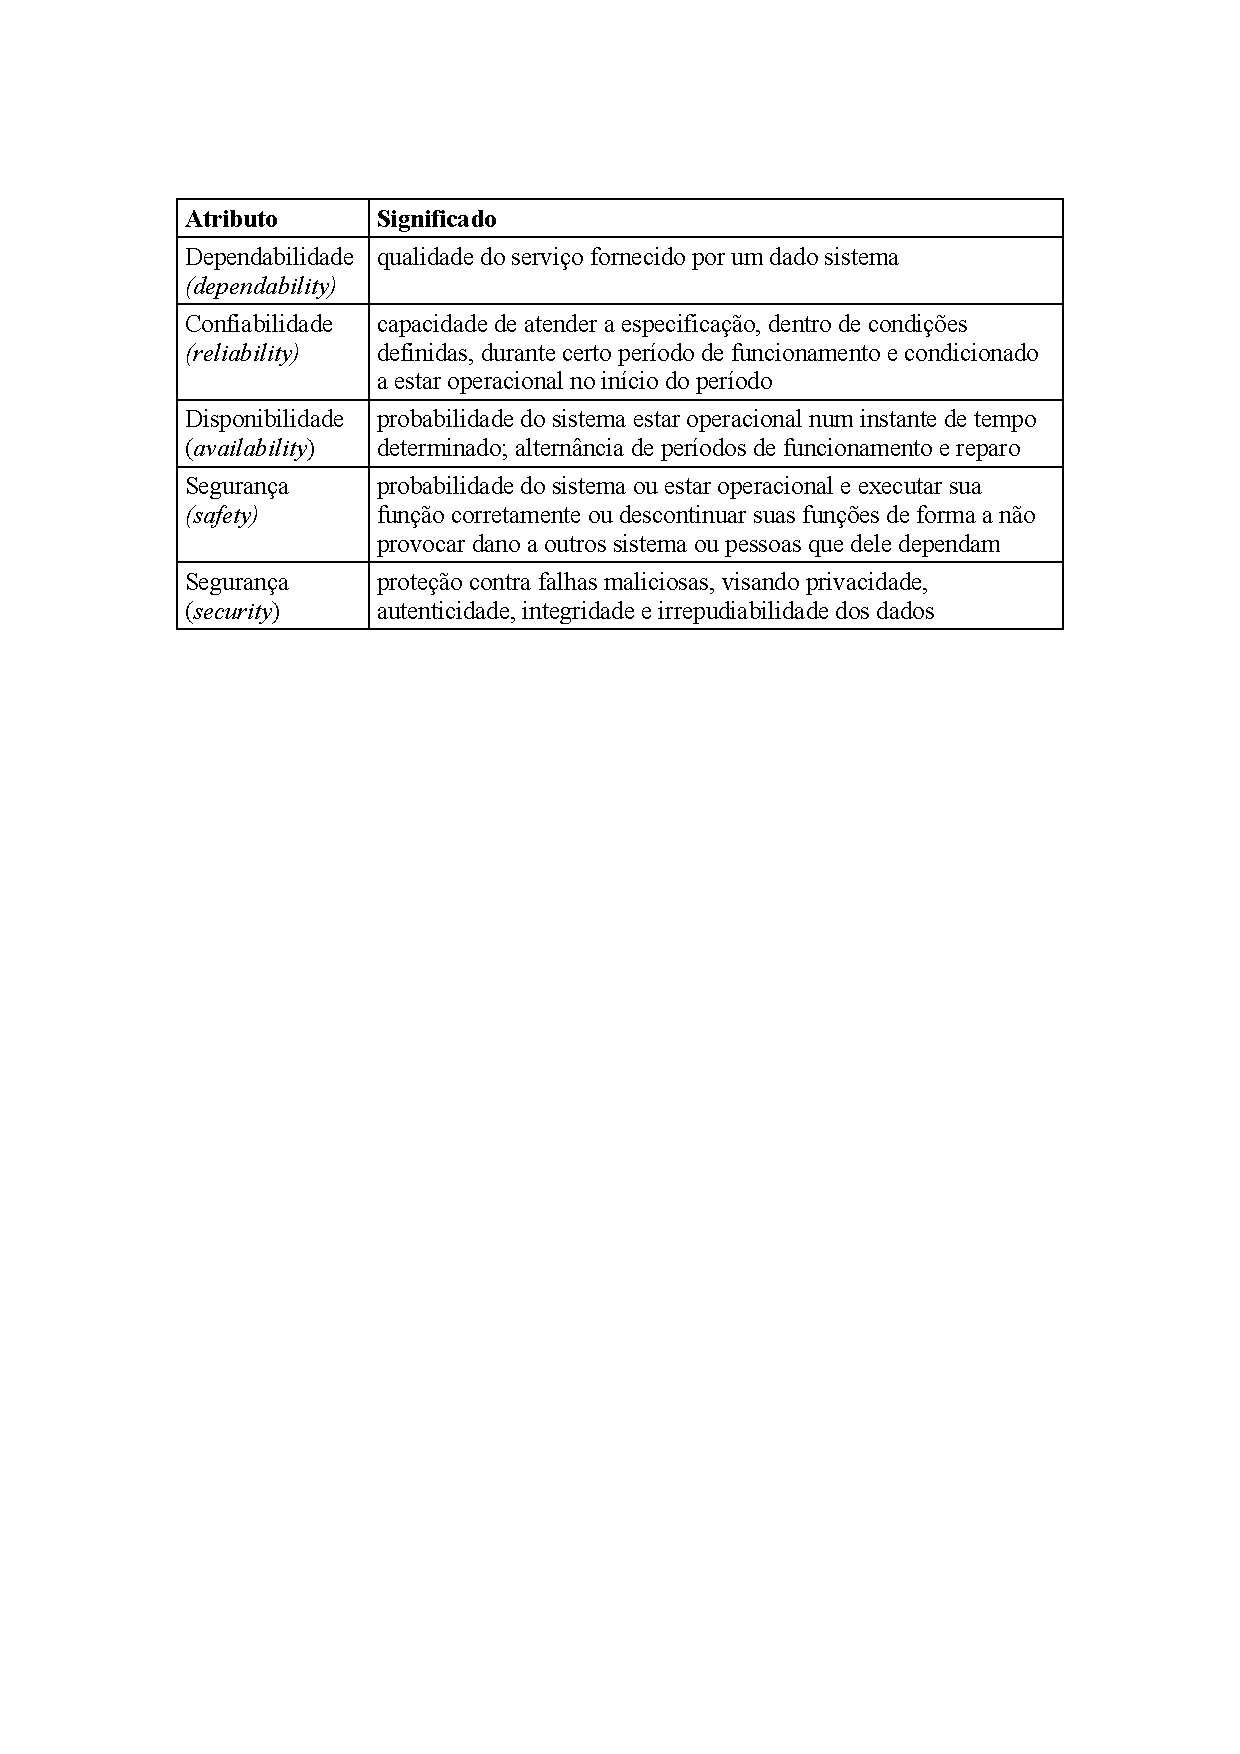
\includegraphics[height=3in]{figuras/tabela_weber.pdf}

\end{center}
\end{table*}
% subsection dependabilidade (end)

Os conceitos apresentados ao longo dessa seção servem como base para compreendermos as técnicas de tolerância a falhas em computação ubíqua e as sutis variações que surgem quando da aplicação de técnicas básicas a ambientes móveis e ubíquos.

\section{Falhas em Ambientes Ubíquos}
\label{sec:falhas_ubicomp}
Os componentes que integram um sistema ubíquo são peças de software e hardware cuja confiabilidade não é garantida. Componentes de software podem não ter sido suficientemente testados ou sua especificação pode não ter coberto todas as excessões que seus algoritmos poderiam gerar, como já vimos na seção anterior. Além disso, falhas podem estar inseridas nos mais variados segmentos de um sistema ubíquo. Dispositivos que dependem de baterias, como laptops e telefones celulares, não podem ser considerados totalmente confiáveis. A interoperabilidade entre dispositivos é uma questão que também gera problemas de confiança nestes sistemas. Falhas de conectividade pelas mais diversas razões, muitas das quais o sistema não pode controlar (como um usuário que leva um dispositivo para fora da área de cobertura de sinal), também reduzem a confiabilidade do sistema. Os serviços básicos de aquisição e processamento de contexto, arquivos, notificações, etc. podem também ser a origem de falhas em sistemas ubíquos.

A seguir desmembraremos as falhas que podem ocorrer em um sistema ubíquo em quatro categorias: falhas nos \textbf{dispositivos}, nas \textbf{aplicações}, na \textbf{rede} e nos \textbf{serviços}. No restante da seção cada uma dessas categorias será coberta em profundidade. Ao final serão apresentadas possíveis implicações das falhas debatidas ao longo da seção.

\subsection{falhas nos dispositivos} % (fold)
\label{sub:falhas_nos_dispositivos}

Um sistema ubíquo geralmente é composto por uma variada gama de dispositivos: computadores \emph{desktop}, \emph{laptops}, dipositivos embarcados, sensores, \emph{smartphones}, câmeras, diplays, projetores, etc. Cada dispositivo de um sistema ubíquo pode gerar suas próprias falhas. Dispositivos móveis, por exemplo, podem ficar sem bateria, sofrer problemas com o sinal e ficar com a conectividade limitada ou nula. Como vimos anteriormente, dispositivos podem ainda, ao invés de parar de funcionar, entregar resultados errados, tipo de falha à qual nos referimos como maliciosa ou \emph{bizantina}.

% subsection falhas_nos_dispositivos (end)

\subsection{falhas nas aplicações} % (fold)
\label{sub:falhas_nas_aplicacoes}

Desenvolver software confiável é, sabidamente, um processo bastante formal e custoso, mas, ainda assim, propenso a falhas. As estapas de teste, verificação e validação chegam a representar metade do custo total do software~\cite{hailpern2002software}. Na verdade, sistemas ubíquos podem ser compostos por aplicações de prateleira que não passaram por um processo de desenvolvimento rigoroso e, embora funcionem bem sozinhas, não interoperam corretamente com outros componentes do sistema. Aplicações podem falhar por diversos motivos como bugs de programação, excessões não capturadas, erros no sistema operacional e até mal uso. Sistemas ubíquos podem também ser alvo de ataques com vírus e \emph{worms}, podendo resultar em falhas \emph{bizantinas} ou interrupção do serviço de um dispositivo

% subsection falhas_nas_aplicações (end)

\subsection{falhas na rede} % (fold)
\label{sub:falhas_na_rede}

A espinha dorsal de um sistema ubíquo é a rede de comunicação. Dispositivos estão interconectados com ou sem fio, e sistemas ubíquos devem munir-se contra falhas na rede causadas por fraqueza do sinal, dispositivos que saem da área de cobertura e tornam-se inalcançáveis, congestionamento devido ao alto tráfico de dados na rede, etc., situações estas que devem ser encaradas como normais de um sistema móvel. Um problema maior ocorre quando uma falha de rede (como um dispositivo que se torna inalcançável) é percebida como uma falha de dispositivo. A identificação automática do tipo de falha é uma questão importante nos sistemas ubíquos.

% subsection falhas_na_rede (end)

\subsection{falhas nos serviços} % (fold)
\label{sub:falhas_nos_servicos}
O sistema ubíquo oferece aos seus usuários um conjunto de serviços, os quais podem ser vistos em duas categorias: serviços básicos e adicionais. Dentre os serviços básicos que um sistema ubíquo deve fornecer estão serviços de descoberta, de nomes e de eventos. Alguns sistemas devem fornecer como básicos serviços de contexto, para aquisição e interpretação de informações contextuais no sistema, e sistemas de arquivos distribuídos, para permitir o acesso ubíquo aos dados. Falhas nos serviços podem ocorrer por \emph{bugs}, erros de sistema operacional, e incluir problemas como sensoriamento/interpretação errada de contexto e perda de eventos. Falhas nos serviços podem fazer com que o sistema ubíquo inteiro pare de funcionar.

% subsection falhas_nos_serviços (end)

\subsection{implicações das falhas} % (fold)
\label{sub:implicacoes_das_falhas}

Ambientes de computação ubíqua são focados principalmente na interface de um ambiente físico com o usuário, tentando fazer como que os dispositivos sejam ``invisíveis'' e operem com a menor interveção do mesmo. Assim, a ocorrência de uma falha neste tipo de sistema pode ser desde algo irritante, que diminuirá sua aplicabilidade, até algo perigoso, que coloque a vida de algum usuário em risco.

\subsubsection*{Dores de cabeça}

Consideremos uma casa inteligente~\cite{Kidd99} onde, assim que o morador entra, sua presença é identificada e o ambiente automaticamente configurado para ele. A temperatura é ajustada, seu canal de TV preferido é acionado em algum display, a iluminação é ajustada pelo acendimento de lâmpadas e fechamento de janelas, tudo isto de forma automática. Caso esse sistema falhe, na melhor das hipóteses, causará no morador uma irritação momentânea. Mas, por exemplo, o sistema pode errar ao identificar um morador e ativar as configurações de outro usuário, eventualmente liberando acesso restrito a informações deste. Além disso, caso as falhas sejam intermitentes, o usuário precisará procurar o origem da falha e tentar corrigí-la, o que pode ser uma tarefa árdua em um ambiente com centenas de dispositivos interconectdados para oferecer serviços em cooperação. Ainda, o fato de fazer manutenção em um determinado dispositivo pode implicar em falhas de outros dispositivos que estejam funcionando corretamente, mas dependam do primeiro para continuar fornecendo algum tipo de serviço.

\subsubsection*{Risco de morte}

Sistemas ubíquos para a área médica formam é área de aplicação da computação ubíqua onde falhas podem ser catastróficas. Basicamente, espera-se que tais sistemas monitorem pacientes, identifiquem problemas e solicitem assistência médica automaticamente. Falhas em sensores de monitoramento ou no sistema de notificação, por exemplo, podem resultar em danos severos à saúde do paciente. A vida de pacientes depende fortemente destes sistemas, logo estes devem ser altamente dependáveis.

\subsubsection*{Prejuízos e quebras de segurança}

A não identificação de uma falha no sistema é, também, fonte de perigo em um sistema ubíquo. Problemas de sensoriamento podem levar ao superaquecimento ou super-resfriamento de um ambiente de temperatura controlada, acarretando na perda de alguma cultura vegetal ou mercadoria refrigerada, por exemplo. A classificação incorreta da falha é outra fonte de problemas. Por exemplo, problemas na identificação de indivíduos pode levar tanto a quebras de segurança quanto a alarmes falsos.

\subsubsection*{Problemas de contexto}

O contexto inclui qualquer informação útil sobre as caraterísticas do ambiente e dos usuários. Podemos ter diversos dispositivos, os quais  podem falhar, para realizar a aquisição de informação contextual: câmeras, sistemas de reconhecimento de voz, sensores de movimento, de temperatura, RFIDs, etc. Informações contextuais são usadas para adaptar proativamente o ambiente ubíquo às necessidades de seus usuários. Um grande desafio aqui é aumentar a robustez na inferência de informação contextual. Diversas técnicas fundem informações contextuais capturadas por diversas fontes para construir uma visão de contexto de mais alto nível, porém nem sempre conseguem criar regras claras de inferência sobre essas abstrações. Problemas na aquisição e inferência de informações contextuais podem levar a um configuração errônea do ambiente físico e levar diversos problemas já enumerados, desde má regulagem da temperatura ambiente até quebras no sistema de segurança.

% subsection implicaçoes_das_falhas (end)





\section{Abordagens para Tolerância a falhas em ambientes ubíquos}
\label{sec:tolerancia}
A área de tolerância a falhas tem evoluído através de décadas de pesquisa nas mais diversas áreas como sistemas operacionais, redes de computadores, arquitetura de computadores, etc. Contudo, cada pequena nova área da computação propõe um novo cenário com novos desafios, fazendo com que as técnicas já desenvolvidas tenham aplicabilidade limitada. Esta seção apresenta estratégias para a identificação e o tratamento das falhas geradas no contexto de sistemas ubíquos.

\subsection{Identificação de Falhas} % (fold)
\label{sub:identificacao}

A identificação de falhas é uma tarefa árdua em sistemas ubíquos onde uma miríade de dispositivos pode estar conectada de forma complexas e escondidas do usuário. Por exemplo, para saber se um certo dispositivo parou, pode-se empregar alguma técnica de \emph{timeout} como \emph{heartbeat messages} (mensagens de ``batimento cardíaco''). Um dispositivo deve periodicamente enviar tais mensagens para o componente detector de falhas, de forma que este possa identificar quando um dispositivo pare de funcionar corretamente. Contudo, em um sistema com um grande número de dispositivos, \emph{heartbeat messages} podem adicionar significativos tráfego na rede e carga de trabalho no detector de falhas. Além disso, um dipositivo que se torna inalcançável na rede pode levar o detector de falhas a uma interpretação errônea, de que o dispositivo parou de funcionar corretamente.

Falhas bizantinas, assim como em qualquer área da computação, são um problema maior ainda. Mesmo os dispositivos que não param de funcionar podem, por exemplo, seguir enviando \emph{heartbeat messages} regularmente, mas responder de forma errada as requisições. Em um sistema ubíquo, falhas bizantinas podem resultar em inferência errada de informação contextual e uso inapropriado de recursos, como visto anteriormente.

A contenção de falhas é um assunto que ganha importância em sistemas ubíquos, dado que estes podem ser compostos por uma vasta gama de dispositivos, os quais devem trocar informações com frequência, podendo rapidamente propagar um erro para o restante do sistema. Podemos considerar um espaço inteligente que se configura de acordo com os indivíduos que estão presentes: uma falha em um RFID pode levar a uma identificação errônea de um indivíduo, o que fará com que o ambiente se configure da maneira errada, por exemplo.

% subsection identificação_de_falhas (end)

\subsection{Contornando as Falhas} % (fold)
\label{sub:contornando_as_falhas}

Como dissemos na Seção~\ref{sec:falhas_comp}, essencialmente, todos os mecanismos de tolerância a falhas envolvem a replicação de algum recurso, seja hardware, sotware, informação, e ainda temos a redundância temporal, onde o sistema fica armazenando seu estado de tempos em tempos para recuperar-se de alguma falha transiente. Discutiremos a seguir algumas destas técnicas de tolerância a falhas aplicadas a ambientes de computação ubíqua.

\paragraph{Reiniciar aplicações} % (fold)

Quando uma falha é detectada em um processo, a técnica mais simples vale também em um abiente ubíquo: reiniciar o processo. Para minimizar a computação e tornar a reexecução menos perceptível ao usuário, deve-se empregar redundância temporal, ou seja, o estado do processo é armazenado periodicamente e recuperado em caso de reinício por falha. Esta técnica é bastante útil e diversas aplicações a empregam em cenários ubíquos

% paragraph reiniciar_aplicações (end)

\paragraph{Dispositivo suplente} % (fold)

Quando erros em uma determinada aplicação são gerados por falhas no hardware, esta aplicação deve ser escalonada em um dispositivo que forneça a mesma funcionalidade, ou funcionalidades mínimas necessárias para a aplicação. Caso o dispositivo suplente não suporte a execução da apliacação que falhou, outra aplicação que forneça funcionalidade semelhante pode ser ativada. Por exemplo, caso acabe a bateria do \emph{smartphone} do usuário e este estava tocando uma certa música, recuperada dos dados do usuário com acesso ubíquo, o sistema pode seguir tocando a mesma música em algum aparelho presente na peça, por exemplo, o \emph{laptop} do usuário. Questões de disponibilidade, privacidade e securança devem ser considerados neste caso.

% paragraph dispositivo_suplente (end)

\subsection{Notificando falhas} % (fold)
\label{sub:notificando_falhas}

Há situações em que uma falha não pode ser contornada sem intervenção de um usuário do sistema. Nestes casos o sistema deve prover um mecanismo de relatório de falhas ao usuário, de forma que este possa tomar a decisão cabida. Este mecanismo deve ser o menos intrusivo possível, ou seja, deve desviar o usuário o mínimo possível de sua real tarefa que, obviamente, não é consertar problemas no sistema. Falhas podem ser reportadas por displays, alto-falantes e qualquer outro meio perceptível pelo usuário. A maneira correta de reportar falhas em um sistema ubíquo pode depender da sua aplicação específica e ainda é um tema de pesquisa pouco explorado.

% subsection notificando_falhas (end)

\textbf{Falar de NoC e self-healing routers} (paper do ROBUST)


\section{Estudos de Caso}
\label{sec:estudos}
Diversos trabalhos têm surgido na academia propondo aplicações práticas de computação ubíqua. No entanto, cada domínio de aplicação possui suas peculiaridades e apresenta seu modelo de falhas característico. Esta seção destina-se a apresentar estudos de caso da academia onde soluções gerais e específicas são empregadas no sentido de tolerar falhas nestes sistemas.

\subsection{CoBrA} % (fold)
\label{sub:cobra}

CoBrA (\emph{\textbf{C}ontext \textbf{Br}oker \textbf{A}rchiecture}) é um \emph{middleware} de computação ubíqua que fornece serviços básicos para a aquisição e gerenciamento de informação contextual em espaços inteligentes (\emph{smart spaces}). O objetivo de CoBrA é permitir que agentes distribuídos em um ambiente ubíquo possam acessar um modelo compartilhado de contextos, contribuir com informações para este modelo e gerenciar o acesso de terceiros a suas informações contextuais em um ambiente ubíquo com sensibilidade o contexto.

CoBrA possui uma arquitetura \emph{broker-centric}, ou seja, existe um agente central (\emph{broker}) que faz inferências sobre as informações contextuais dos demais agentes do ambiente e serve como intermediário de todas as trocas de informações contextuais entre os demais agentes. Podemos ainda ter redes de \emph{brokers} trocando informações contextuais sobre os agentes presentes em seus respectivos espaços inteligentes, como é o caso do sistema ubíquo EasyMeeting~\cite{finin2005semantic}, ilustrado na Figura~\ref{fig:_cobra_easy_meeting}, sistema este construído sobre o CoBrA.

\begin{figure}[htbp]
	\centering
		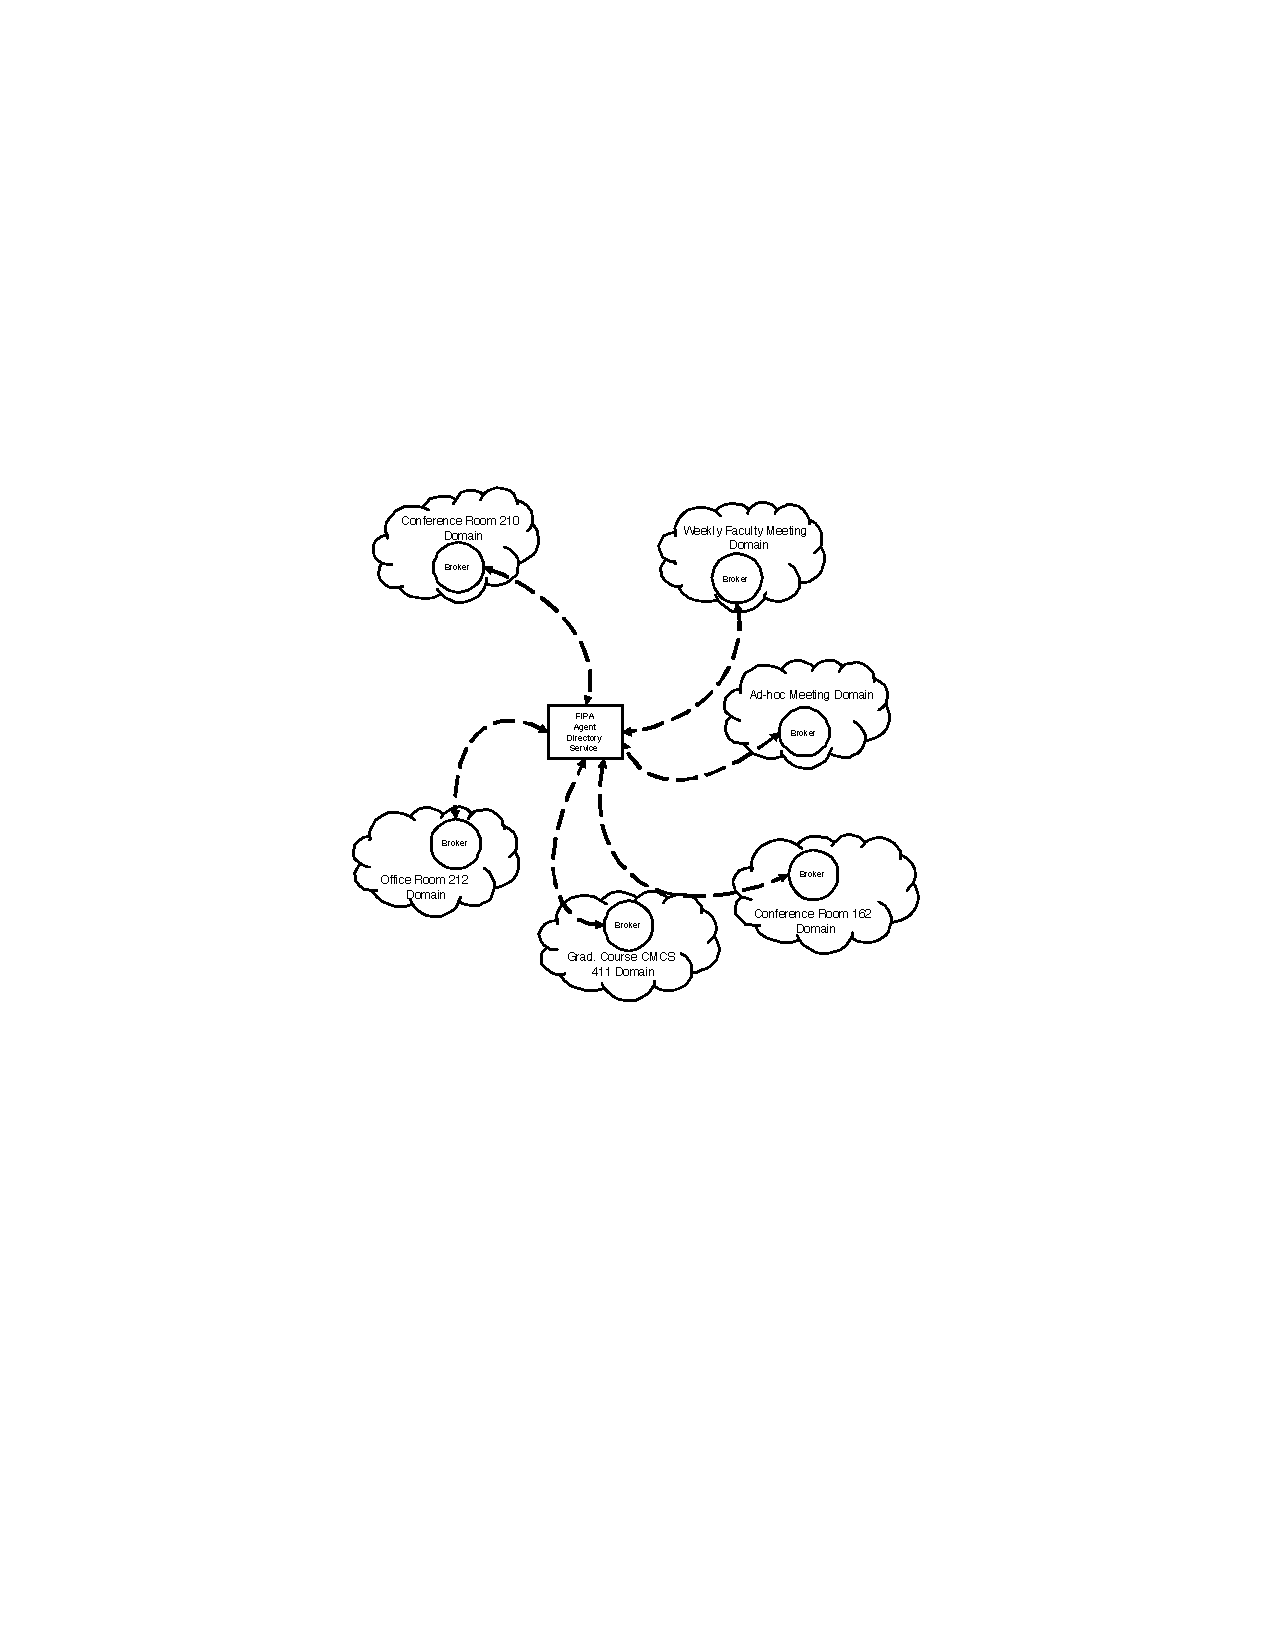
\includegraphics[width=.7\textwidth]{figuras/cobra_easy_meeting.pdf}
	\caption{EasyMeeting: estudo de caso desenvolvido sobre CoBrA.}
	\label{fig:_cobra_easy_meeting}
\end{figure}

CoBrA propõe mecanismos de tolerância a falhas baseados na arquitetura proposta em~\cite{kumar2000adaptive} sobre \emph{times persistentes de brokers}. Tal arquitetura proposta (\emph{Adaptive Agent Architecture}) assume que para um \emph{broker} ingressar em um time, este deve assumir comprometimentos em relação aos serviços que devem prestar, o que facilita a substituição de um \emph{broker} que apresenta falhas e faz com que o sistema forneça funcionalidades básicas enquanto houver pelo menos um \emph{broker} funcionando. Outros comprometimentos que os \emph{brokers} podem assumir lhes dão a permissão para criar/escolher novos \emph{brokers} e incluí-los no time, fazendo com que o sistema consiga se adaptar automaticamente perante variações no ambiente, tais como falhas nos agentes. 

A teoria que embasa estes mecanismos é a \textbf{teoria das intenções conjuntas} (\emph{theory of joint intentions}), amplamente utilizada em ramos da computação ligados à Inteligência Artificial. Este conjunto de técnicas espera, intuitivamente, que um time será mais robusto do que um conjunto de indivíduos. A premissa básica é de que um time trabalha junto para atingir uma determinada meta (por exemplo, prover serviços de contexto). Quando um membro do time está com problemas outros membros do time o ajudarão (por exemplo, um servidor pode ordenar o reinício de um outro servidor que apresenta uma falha transiente e restaurar seu estado) e quando um membro ficar indisponível o restante dos membros farão seu trabalho para cumprir as metas do time (por exemplo, chamadas ao servidor indiponível podem ser atendidas por um outro servidor qualquer do time). Um time deixará de cumprir uma meta global se, e somente se, todos os membros escolherem esta opção. Logo, times são organizações inerentemente tolerantes a falhas.

Em~\cite{kumar2000adaptive} são detalhadas estratégias necessárias para implementar os mecaninsmos de times em software, inclusive os protocolos de comunicação que devem ser usados para a autocoordenação dos times de \emph{brokers}.

% subsection cobra (end)

\subsection{Coda FS} % (fold)
\label{sub:coda_fs}

O Coda File System~\cite{satyanarayanan1990coda} é um sistema de arquivos distribuído descendente do Andrew File System (AFS)~\cite{howard1988overview} e fornece diversos recursos semelhantes aos do AFS. Coda foi projetado para ser um sistema de arquivos escalável, seguro e altamente disponível, com alto grau de transparência de distribuição. Tomando também em consideração a alta disponibilidade, os projetistas do Coda tentaram chegar a um alto grau de transparência na recuperação de falhas. Para obter algum grau de transparência de recuperação de falhas os desenvlovedores do Coda criaram vários mecanismos sofisticados baseados em cache de dados no lado do cliente e replicação de servidores de arquivos.

\subsubsection*{Operação desconectada}

Os clientes Coda, ao contrário de clientes NFS, por exemplo, continuam a operar normalmente mesmo sem conseguir conectar nenhum dos servidores~\cite{kistler1992disconnected}. Uma vez que o cliente abre um arquivo do servidor, este  passa a editar uma cópia local, de forma que, quando o usuário terminar sua sessão sem conexão, não resultará em erro algum. Quando as alterações forem atualizadas no(s) servidor(es), no entanto, pode ser que ocorra algum conflito, o qual nem sempre é resolvido automaticamente. Porém raramente os usuários compartilham um arquivo para escrita, tornando esta situação uma exceção.

Para que a operação desconectada realmente funcione, todos os arquivos que o cliente precisa devem estar em cache. Coda provê um mecanismo sofisticado chamado \emph{hoarding} para garantir isso. O mecanismo funciona como segue. Primeiro, um usuário pode criar uma lista dos arquivos que o mesmo julga serem os mais importantes para ele (\emph{hoard database}). O Coda usa esta lista fornecida pelo usuário juntamente com a localidade de referência aos arquivos para atribuir prioridades a estes. Uma vez que foram atribuídas prioridades a todos os arquivos do usuário, o Coda se vale de três regras básicas para gerenciar a cache:

\begin{enumerate}
	\item Não existe nenhum arquivo fora da cache com prioridade maior que a de um que está na cache;
	\item Ou a cache está cheia ou nenhum arquivo fora da cache tem prioridade não-zero;
	\item Cada arquivo em cache é somente uma cópia de um arquivo no servidor.
\end{enumerate}

Para o Coda, se a cache satisfaz estas 3 regras ela está em estado de \emph{equilibrium}. Contudo as prioridades podem ser alteradas dinamicamente. Para reestabelecer o \emph{equilibrium} da cache, a cada 10 minutos o módulo cliente realiza o que os autores chamam de \emph{hoard walk}, reajustando prioridades e substituindo arquivos na cache. Contudo, embora estas técnicas tenham aumentado muito a eficiência do Coda FS, elas não garantem que todos os dados que o cliente precisará futuramente estarão armazenados em cache no caso de uma operação desconectada.

\subsubsection*{Memória Virtual Recuperável}
Além de prover alta disponibilidade com as operações desconectadas, Coda emprega um mecanismo que facilita a recuperação de um processo em falha. Memória Virtual Recuperável (\emph{Recoverable Virtual Memory} -- RVM) é um mecanismo que armazena estruturas de dados cruciais da a aplicação para uma recuperação rápida em caso de falha (mais detalhes em~\cite{satyanarayanan1994lightweight}).

A ideia do RVM é bastante simples. As estruturas de dados mais importantes da aplicação são mantidas em um espaço conhecido da memória principal e são armazenados logs para cada alteração nestes dados, de maneira semelhante a um esquema de transações, porém sem suporte a concorrência. Em caso de falha de um processo, os dados são restaurados de maneira relativamente fácil através do log de operações nas estruturas de dados mais importantes.

O Coda FS ainda implementa diversos mecanismos de segurança que aumentam ainda mais a confiabilidade dos usuários neste sistema de arquivo.

% subsection coda_fs (end)

\subsection{Prism-MW} % (fold)
\label{sub:prism_mw}

Prism-MW~\cite{Seo07} é uma plataforma de \emph{middleware} que oferece um conjunto de blocos básicos para a construção de sistemas ubíquos. O Prism-MW fornece mecanismos de tolerância a falhas embutidos, ao mesmo tempo que sua arquitetura é eficiente e clara. O \emph{middleware} arquitetural é, basicamente composto por 3 camadas. Na base uma Máquina Virtual, que permite a implantação do sistema em plataformas hetereogêneas sem modificações na implementação. Acima da máquina virtual são fornecidos os blocos básicos de construção da arquitetura (componentes, conectores, eventos, etc.). No topo, usando os componentes da camada arquitetural, são implementados três serviços considerados essenciais para sistemas ubíquos: $(1)$ descoberta dinâmica de novos serviços e recursos, $(2)$ recuperação automática e transparente de falhas e $(3)$ determinação analítica das estratégias de replicação de componentes e arquiteturas de implantação.

\begin{figure}[htbp]
	\centering
		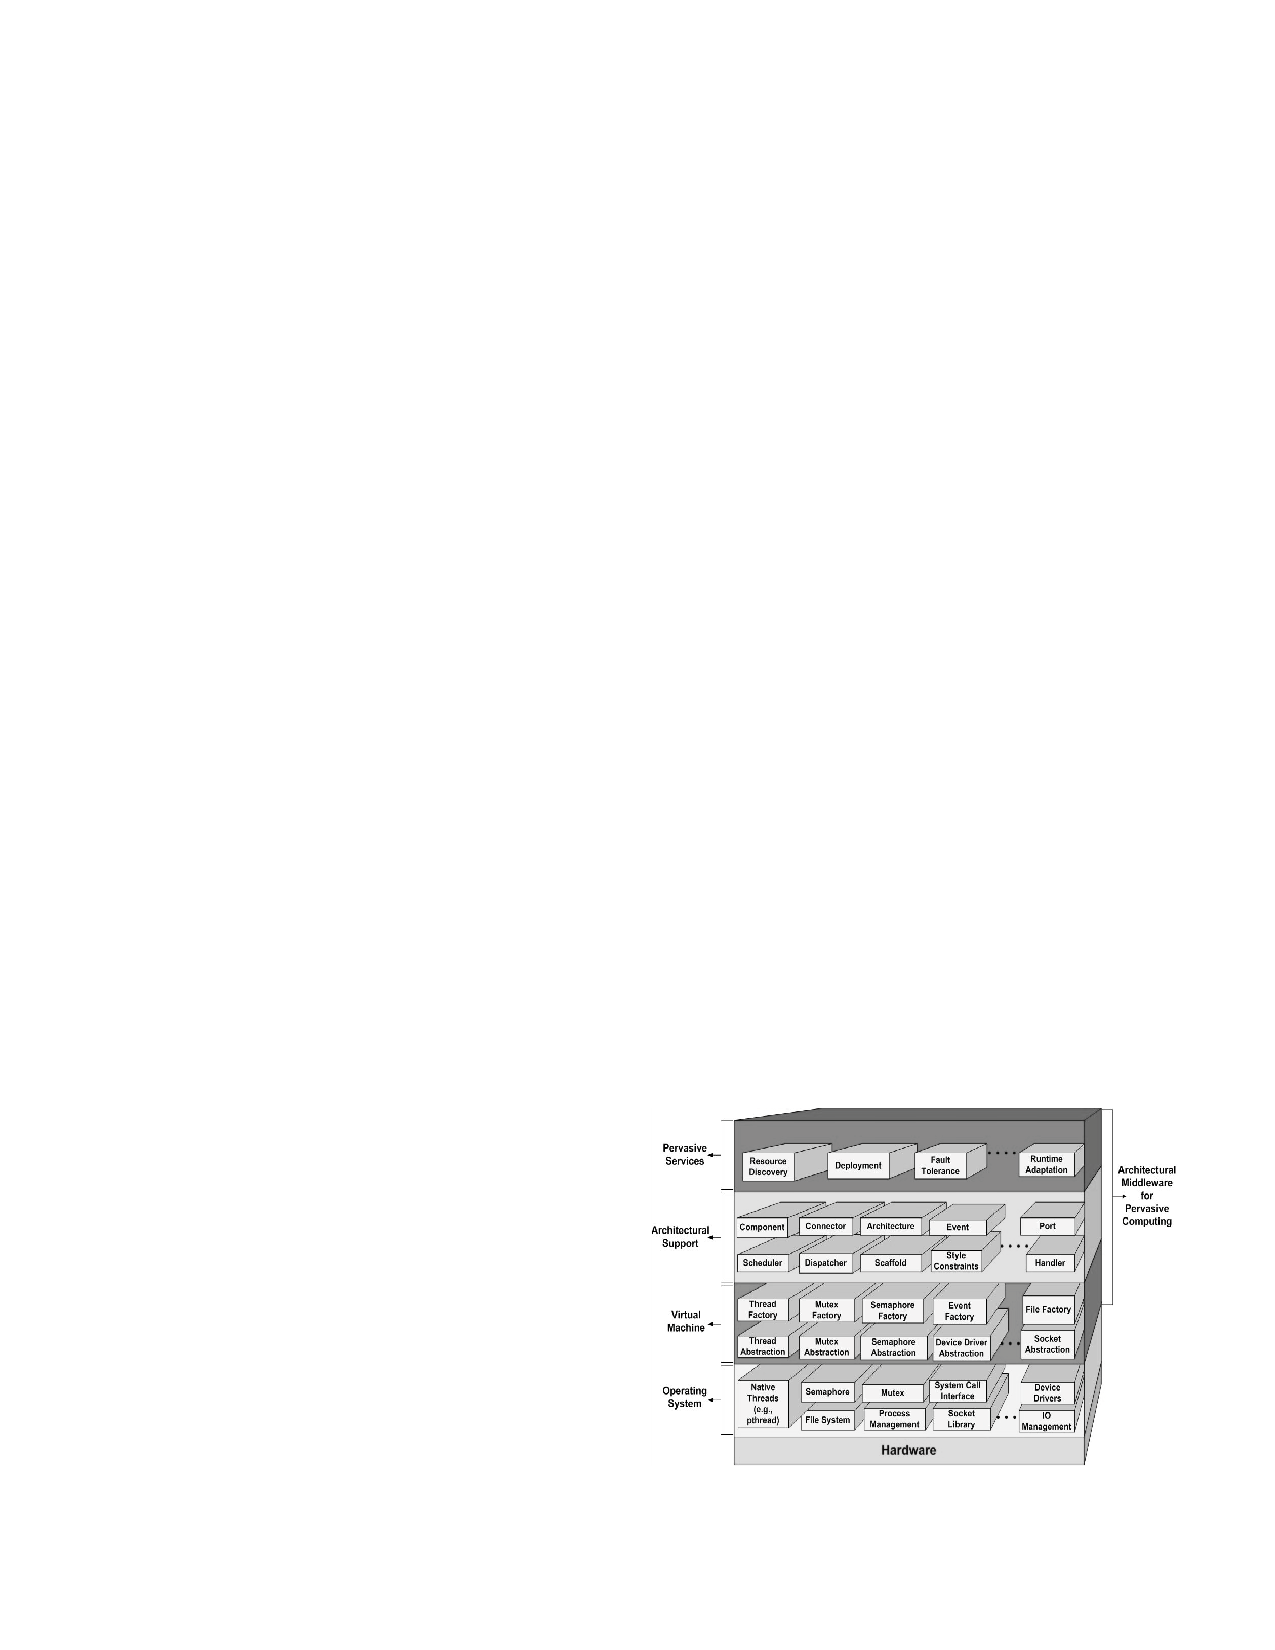
\includegraphics[width=.7\textwidth]{figuras/prism.pdf}
	\caption{Visão geral do \emph{middleware} Prism.}
	\label{fig:prism}
\end{figure}

Como pode ser visto na Figura~\ref{fig:prism} a abordagem do Prism-MW consiste em separar totalmente a lógica da aplicação da lógica de tolerância a falhas, fornecendo esta última como um serviço da camada superior da arquitetura. Esta abordagem consiste basicamente em fornecer \textbf{conectores lógicos} entre os componentes, que oferecem diferentes garantias para os diferentes elementos que irão conectar-se através deles, e módulos que auxiliam no \textbf{gerenciamento de componentes replicados}. A abordagem de Prism auxilia na tarefa de construção, análise e adaptação de software ubíquo mantendo a qualidade de serviço (QoS) em diversos cenários ubíquos~\cite{Seo07}.

% subsection prism_mw (end)

% \subsection{ADRF} % (fold)
% 
% \emph{Assured Dynamic Reconfiguration Framework} (ADRF) é um \emph{framework} qua fornece recursos básicos para a reconfiguração de um sistema ubíquo. 

% subsection adrf (end)

% \subsection{GaiaOS} % (fold)
% \label{sub:gaiaos}
% 
% O projeto Gaia consiste de uma plataforma semelhante a um sistema operacional para ambientes ubíquos, que fornece um mecanismo de abstração do acesso aos recursos físicos presentes em um espaço inteligente. Diversos conceitos presentes em sistemas operacionais modernos, como eventos, sinais, sistemas de arquivos e processos, são traduzidos no GaiaOS para o contexto da computação ubíqua. A Figura~\ref{fig:figuras_gaiaos} fornece uma visão geral dos componentes em um sistema GaiaOS. Como pode-se observar nesta ilustração, o \emph{Unified Object Bus} é a espinha dorsal do GaiaOS, pois é o barramento pelo qual todos os dispositivos em um espaço inteligente podem se intercomuncar por uma única linguagem.
% 
% \begin{figure}[htbp]
% 	\centering
% 		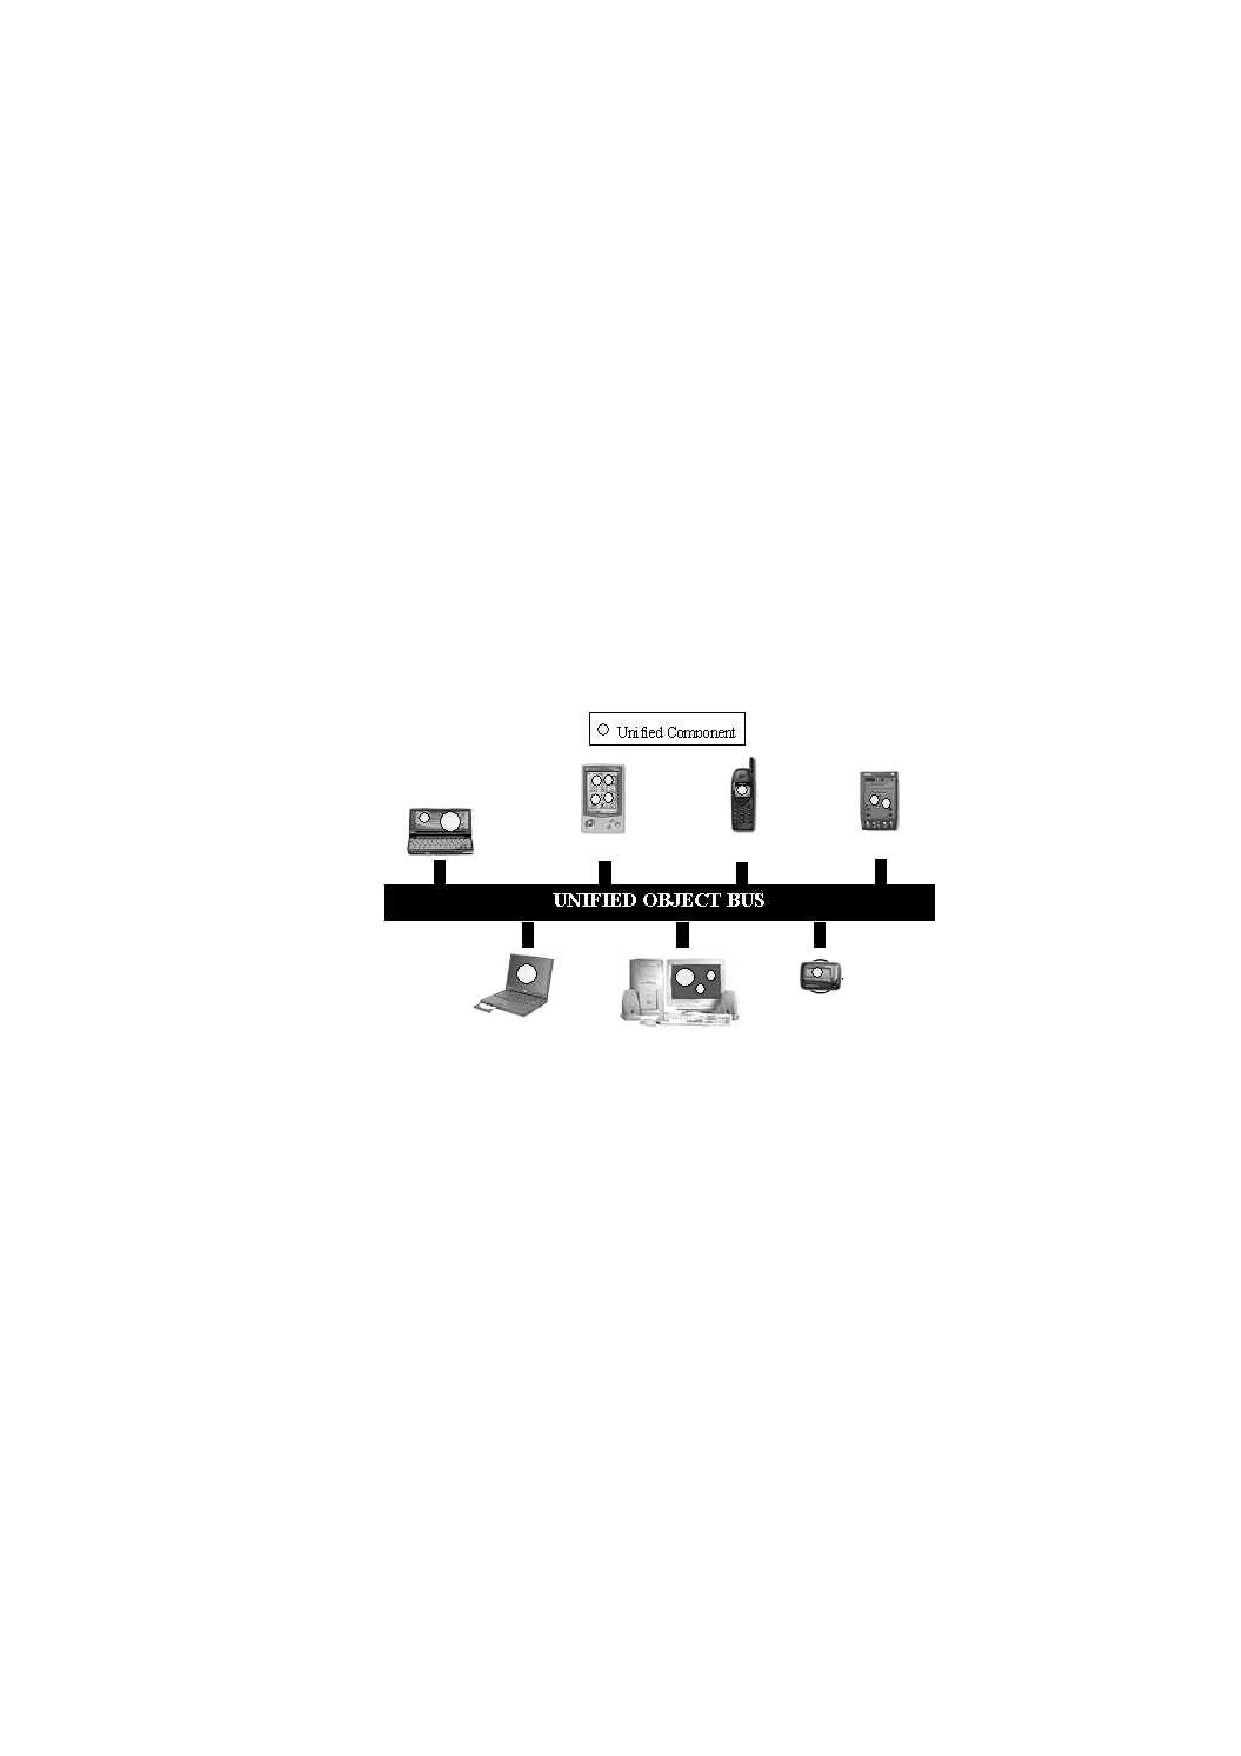
\includegraphics[width=.7\textwidth]{figuras/gaiaos.pdf}
% 	\caption{Visão geral do GaiaOS.}
% 	\label{fig:figuras_gaiaos}
% \end{figure}
% 
% No \emph{kernel} do GaiaOS são implementados serviços de inicialização básica do sistema: gerenciador de eventos; localizador de serviçoos e indivíduos; base de registros de dispositivos; serviços, indivíduos e aplicações ativos no sistema; sistema de arquivos; e serviços de autentitcaçãoo e autorização de usuários.
% 
% A extensão \emph{Gaia Context Infrastructure}~\cite{ranganathan2003middleware} adiciona sensibilidade ao contexto a espaços inteligentes construídos com GaiaOS.
% 
% % subsection gaiaos (end)


\subsection{Soluções de Medicina Ubíqua} % (fold)

A área médica, embora apresente uma enorme demanda por soluções de tolerância a falhas, fornece mais sugestões de soluções para os problemas possíveis em ambientes de medicina ubíqua do que protótipos de fato. O artigo ``\emph{Dependability Issues of Pervasive Computing in a Healthcare Environment}''~\cite{bohn2004dependability} levanta diversos problemas e soluções em medicina ubíqua, principalmente ligados a falhas de segurança, os quais serão discutidos a seguir.

Hospitais geralmente possuem os registros de seus pacientes em um banco de dados, contudo o mecanismo de controle de acesso ao banco de dados não é flexível o suficiente para um ambiente ubíquo, onde o acesso deve ser feito de ``qualquer lugar''. Para obter esta flexibilidade o mecanismo de \emph{controle de acesso} a esse banco de dados deve ser replicado e separado do mecanismo de \emph{gerenciamento} das informações do banco. Contudo, estes servidores de controle de acesso podem falhar. Assim, \emph{pontos de acesso} espalhados pelo hospital devem ``alcançar'' um número $k$ (maior ou igual a 2) de servidores de controle de acesso. A Figura~\ref{fig:pervasive_hospital1} mostra uma possível distribuição de pontos de acesso e servidores de controle de acesso em um ambiente médico ubíquo. Este esquema pode incluir esquemas de tolerância a falhas de segurança que distribuem os certificados digitais dos pontos de acesso entre mais de um servidor de controle de acesso~\cite{rabin1989efficient}, de forma que se um servidor (ou mais, dependendo de $k$) forem atacados com sucesso, ainda não será possível obter o certificado necessário para acessar a base de dados dos pacientes.

\begin{figure}[htbp]
	\centering
		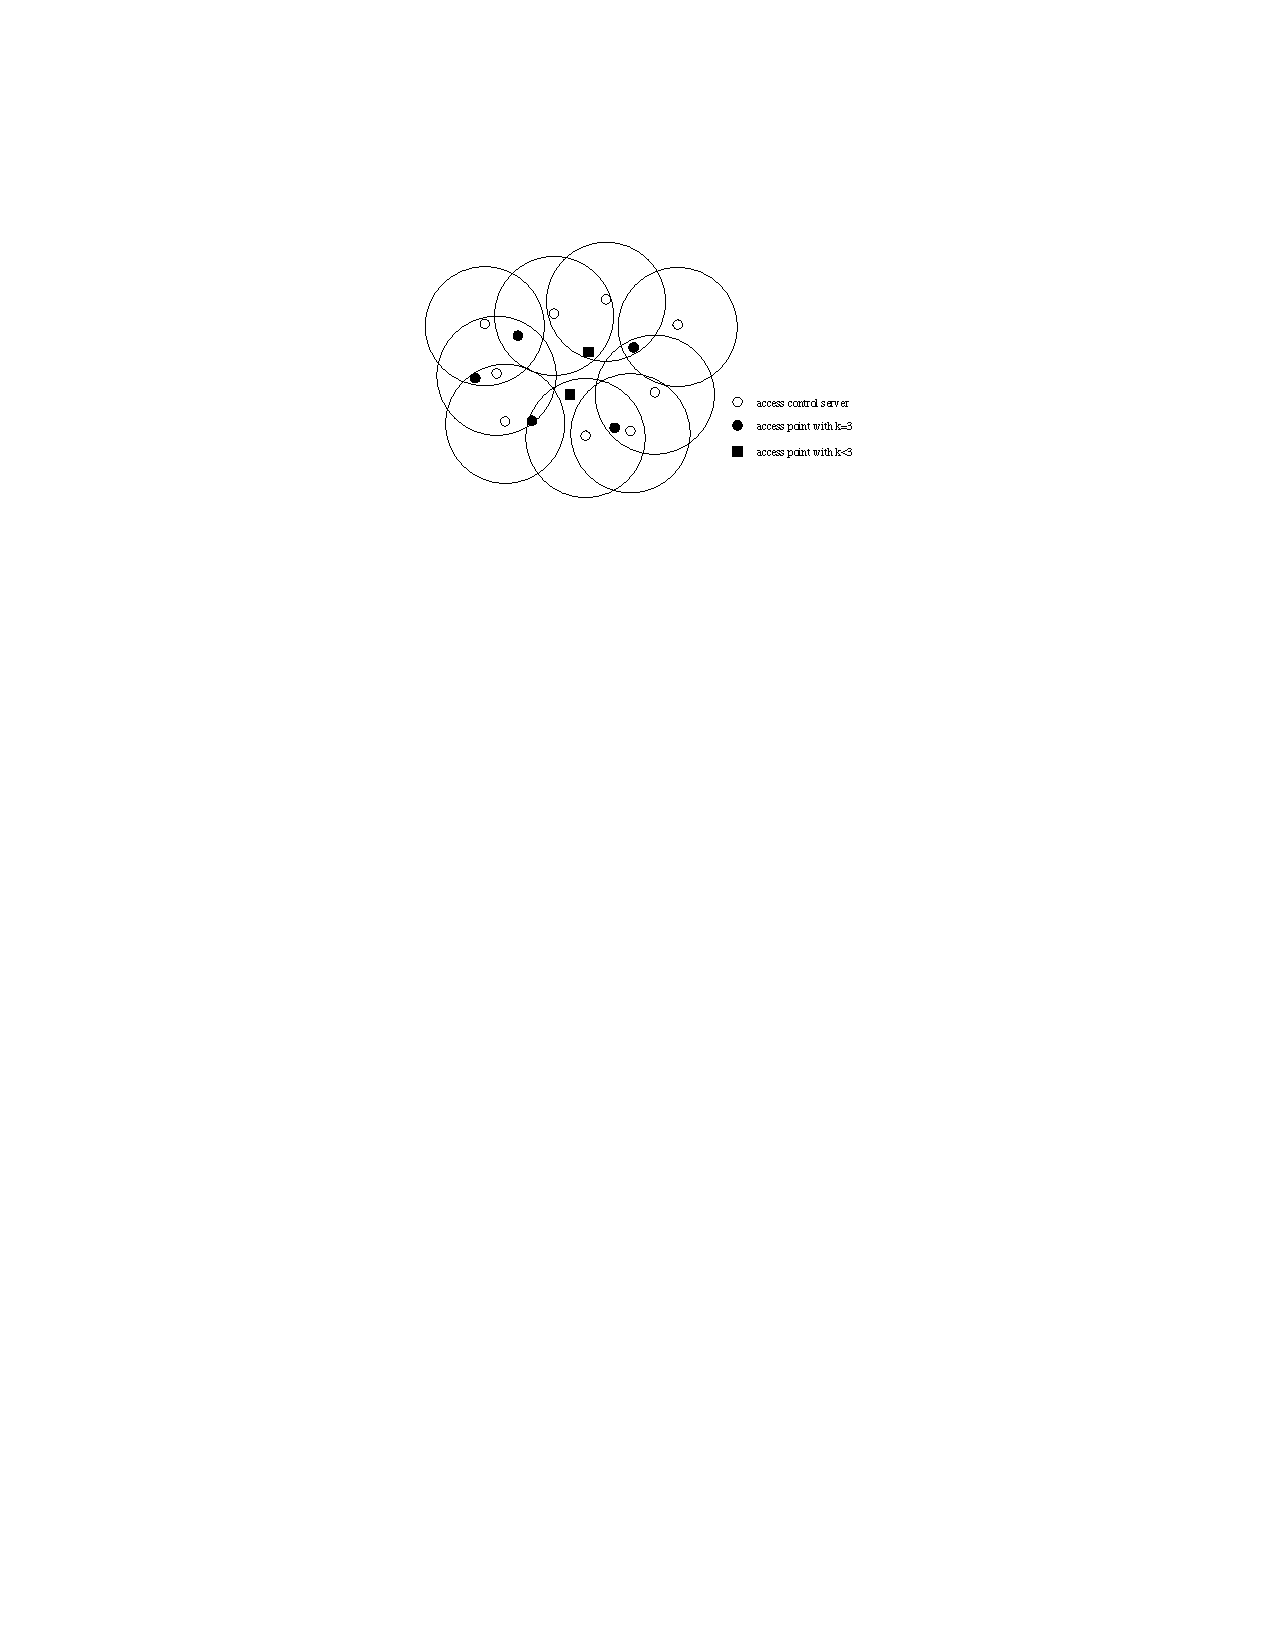
\includegraphics[width=.6\textwidth]{figuras/pervasive_hospital1.pdf}
	\caption{Possível distribuição de pontos de acesso e servidores de controle de acesso em um ambiente médico ubíquo. Círculos pequenos vazados representam servidores de controle de acesso enquanto os círculos maiores representam o alcance de seu sinal. Círculos cheios representam pontos de acesso que ``alcançam'' três servidores, e quadrados cheios representam pontos de acesso que ``alcançam'' menos de três servidores e podem não obter credenciais para acessar o banco.}
	\label{fig:pervasive_hospital1}
\end{figure}

Em um ambiente médico ubíquo, assim como em outros ambientes de computação, é extremamente importante proteger a rede e os computadores do ambiente de uma série de possíveis ataques, como ataques de negação de serviço (\emph{Denial of Service} -- DoS), hackerismos, cavalos de Troia, etc. Serviços de auditoria automática de segurança devem incluir mecanismos básicos~\cite{lunt1988automated,tsudik1990audes}, como detecção de intrusos ou um \emph{firewall}. Em particular, os mecanismos devem ser aprimorados para proteger uma infraestrutura altamente \textbf{heterogênea} e \textbf{distribuída}, como um sistema ubíquo. Por exemplo, um sistema distribuído de detecção de intrusos como proposto em~\cite{bass2000intrusion} consegue lidar com diversos tipos de ataques distribuídos. O próprio serviço de auditoria deve possuir suporte de tolerância a falhas, o que inclui suporte a operações desconectadas~\cite{kistler1992disconnected} para manter o serviço em desconexões transientes. Por exemplo, sensores distribuídos podem ter que \emph{bufferizar} dados durante o período de desconexão da rede.

Além destes fatores, decisões de arquitetura devem ser tomadas de forma aumentar, robutez, escalabilidade e autonomia do sistema médico ubíquo. A ideia é permitir que o sistema seja adaptativo de tal forma que diferentes regiões físicas do sistema funcionem de maneira independente. Por exemplo, um incêncio em uma ala de um hospital, resultando em perdas de pontos e servidores de acesso ubíquo, não deve fazer com que o sistema inteiro interrompa os serviços. Além disso, expandir o sistema deve ser uma tarefa simples.

% subsection questões_de_medicina (end)

Soluções desenvolvidos em outras sub-áreas da computação podem ser interessantes para a computação ubíqua, por exemplo, em~\cite{parikhformally} o autor apresenta um protótipo de arquitetura many-core com NoC (\emph{Network on Chip}) e roteadores autorreconfiguráveis e tolerantes a falhas em nível de \emph{hardware}.


\section{Conclusões}
\label{sec:conclusoes}
Tolerância a falhas é um assunto ainda pouco maduro na área computação ubíqua, em parte devido ao fato da área da computação ubíqua em si ser relativamente nova. Contudo, avanços significativos têm sido alcançados, alguns desses avanços diluídos em aplicações específicas de computação ubíqua que necessitam um ou outro recurso de tolerância a falhas. A maioria dos trabalhos estudados busca identificar um conjunto de técnicas básicas de tolerância a falhas que qualquer sistema de computação ubíqua devem implementar e empacotálas em forma de um \emph{framework} ou um \emph{middleware} para suporte ao desenvolvimento de aplicações ubíquas.

A área da computação ubíqua tem um perfil mais focado na interface do sistema distribuído com o usuário final e na incremental fusão de elementos de computação com ambiente físico. Contudo, para que a ubiquidade seja viável é primordial que o sistema seja tolerante a falhas, pois as pessoas dependerão destes sistemas para tarefas complexas e, muitas vezes, vitais. As ferramentas e técnicas de tolerância a falhas necessitam ainda de um considerável amadurecimento, que certamente se acentuará conforme houver mais demanda comercial por soluções de computação ubíqua.

% \begin{center}
% 	\textbf{Agradecimentos}
% \end{center}
% Gostaria de fazer um agradecimento especial aos irmãos Maurício e Laércio Lima Pilla, pelo contrabando de artigos.
	

\bibliographystyle{sbc}
\bibliography{bibs}

\end{document}